%% LyX 2.3.0 created this file.  For more info, see http://www.lyx.org/.
%% Do not edit unless you really know what you are doing.
\documentclass[12pt,spanish,chapterprefix, numbers=noenddot]{book}
\usepackage{ae,aecompl}
\renewcommand{\familydefault}{\rmdefault}
\usepackage[T1]{fontenc}
\usepackage[utf8]{inputenc}
\usepackage[a4paper]{geometry}
\geometry{verbose,tmargin=2.5cm,bmargin=2.5cm,lmargin=2.5cm,rmargin=2.5cm,headheight=1cm,headsep=1cm,footskip=1cm}
\setlength{\parskip}{\medskipamount}
\setlength{\parindent}{0pt}
\usepackage{babel}
\addto\shorthandsspanish{\spanishdeactivate{~<>}}

\usepackage{amsmath}
\usepackage{amsthm}
\usepackage{makeidx}
\makeindex
\usepackage{graphicx}
\usepackage{setspace}
\usepackage{nomencl}
% the following is useful when we have the old nomencl.sty package
\providecommand{\printnomenclature}{\printglossary}
\providecommand{\makenomenclature}{\makeglossary}
\makenomenclature
\usepackage[unicode=true,pdfusetitle,
 bookmarks=true,bookmarksnumbered=false,bookmarksopen=false,
 breaklinks=true,pdfborder={0 0 0},pdfborderstyle={},backref=false,colorlinks=false]
 {hyperref}

\makeatletter
%%%%%%%%%%%%%%%%%%%%%%%%%%%%%% Textclass specific LaTeX commands.
\numberwithin{equation}{section}
\numberwithin{figure}{section}

%%%%%%%%%%%%%%%%%%%%%%%%%%%%%% User specified LaTeX commands.
%Para que las URLs de la bibliografía se pueda pinchar
\usepackage{url}

%Cabeceras y pies de página
\usepackage{fancyhdr}
\pagestyle{fancy}
\lhead[\rightmark]{}
\rhead[]{\leftmark}
\cfoot{\thepage}

%Para que los índices respeten los espacios de las nuemraciones
\usepackage[tocindentauto]{tocstyle}
\usetocstyle{standard}

%Para que ponga "Índice de Tablas" en vez de "Indice de Cuadros"
\addto\captionsspanish{
\def\tablename{Tabla}
\def\listtablename{\'Indice de tablas}
}

%Para que las páginas en blanco no tengan cabecera ni número de página
\makeatletter
\renewcommand*{\cleardoublepage}{\clearpage\if@twoside \ifodd\c@page\else
\hbox{}%
\thispagestyle{empty}%
\newpage%
\if@twocolumn\hbox{}\newpage\fi\fi\fi}
\makeatother

\AtBeginDocument{
  \def\labelitemii{\(\circ\)}
  \def\labelitemiii{\(\triangleright\)}
}

\makeatother

\usepackage{minted}
\setminted{basicstyle={\ttfamily},
breaklines=true}
\usepackage[bibstyle=nature,citestyle=numeric]{biblatex}
\addbibresource{bibliography.bib}
\begin{document}
\frontmatter

\begin{titlepage}

\begin{doublespace}
\begin{center}

\includegraphics[height=3cm]{Figs/logoURJC}\\
Escuela Técnica Superior de Ingeniería Informática
\par\end{center}
\end{doublespace}

\vspace{4cm}

\begin{center}
{\LARGE{}Memoria del Trabajo de Fin de Grado}{\LARGE\par}
\par\end{center}

\vspace{4cm}

\begin{center}
{\large{}Memoria del Trabajo Fin de Grado}\\
{\large{}en Ingeniería Informática}{\large\par}
\par\end{center}

\vspace{4cm}

\begin{center}
{\large{}Autor: Agustín Daniel Schüler Allub}{\large\par}
\par\end{center}

\begin{center}
{\large{}Tutor: José Francisco Vélez Serrano}{\large\par}
\par\end{center}

\begin{center}
Agosto 2018
\par\end{center}

\end{titlepage}

\chapter*{Agradecimientos}

Quiero agradecer sus consejos a Pablo Viniegra Picazo y a Vanessa
Krebs Carretero.

Quiero agradecer a Jorge Aranda García y a Patricia de Gregorio Ruiz
el tiempo que han compartido conmigo estos 4 años.

Quiero agradecer sus contribuciones a todos los desarrolladores de
software libre que me han proporcionado herramientas para realizar
este trabajo.

Finalmente, quiero agradecer su paciencia a mi familia durante el
transcurso de la carrera.

\chapter*{Resumen}

Lo que se presenta en este Trabajo de Fin de Grado es un conjunto
de servicios apoyados en el estándar HTTP\index{HTTP} (\nomenclature{HTTP}{Hypertext Transfer Protocol})
que tienen como fin ser utilizado por clientes. Comúnmente llamado
API\index{API} (\nomenclature{API}{Application Programming Interface}).
Dicha API está enfocada a atender a aplicaciones cliente de caracter
social.

\tableofcontents{}

\mainmatter

\chapter{Introducción}

En un principio, la idea principal era el desarrollo de una aplicación
web, pero una compañera de la carrera propuso dividirnos la carga
de trabajo que supone dicho desarrollo. Por tanto, opté por la realización
de servicios necesarios para el lado del cliente. Se decidió agregar
un grado más de dificultad a dicha aplicación: El uso de la visión
artificial. Dado que la aplicación web en ultima instancia es una
red social, se decidió usar técnicas de Visión Artificial con el fin
de mejorarla.

A continuación se detallaran tanto aspectos de desarrollo y análisis
como aspectos de diseño, experimentación y métricas.

\section{Motivación}

En particular, siempre quise verme inmerso en el problema de desarrollar
una aplicación web en su totalidad. Normalmente en las diferentes
asignaturas de la carrera, se proponían tareas relacionadas con ello,
pero nunca sentí que se profundizara mucho en el tema. 

Como consecuencia, la búsqueda de documentación de las herramientas
utilizadas y el ser autodidacta, han sido pilares importantes en la
realización del TFG. Aunque cabe destacar que ha sido de los mejores
proyectos en los que me he visto involucrado, sobre todo por la libertad
que me proporcionó mi tutor para poder desarrollar dicho proyecto.

Por otra parte, aparte de un fin persona se quería presentar dicha
aplicación web con alguna mejora. Coincidiendo con la asignatura de
Visión Artificial que hemos tenido este ultimo año, decidimos utilizar
dicho campo para presentar dicha mejora. Se pretende realizar sugerencias
a los usuarios sobre sus amistades cuando proceden a realizar una
publicación en la que se incluye una foto.

Mas adelante se explicará con más detalle. 

\section{Estado del arte}

Por lo dicho anteriormente se pueden intuir las soluciones que pueden
llegar a cubrir el problema que se desea abordar en este Trabajo de
Fin de Grado. 

Como he dicho en la sección anterior, asumí una parte concreta del
desarrollo: Administracion del sistema y la lógica que se encarga
de que la pagina web este en perfecto funcionamiento. Una parte importante
en el desarrollo de una aplicación web (o en una parte de ella) es
escoger correctamente las tecnologias utilizadas. 

En mi caso opté por herramientas con las que tenia soltura y además
que estuviesen a la orden del día. Es importante esto último, dado
que es importante que las herramientas cuenten con una documentación
consistente y se encuentren actualizadas.

\subsection*{Lógica de la aplicación web (BackEnd)}

Actualmente existen multitud de herramientas informáticas que se encarguen
del BackEnd de una aplicación web. Con casi total probabilidad la
más utilizada sea el lenguaje de programación PHP, muchas veces viene
preinstalado en la mayoria de sistemas y el lenguaje se parece bastante
a otros bastante famosos. Además, PHP no se suele utilizar en su versión
regular, se suele utilizar algún framework de dicho lenguaje. En mi
caso conocia CakePHP, proporciona una arquitectura MVC, es de codigo
abierto y además habia trabajado con ello durante el tiempo suficiente
como para tener cierta soltura.

Es necesario nombrar a Java, lenguaje fuertemente tipado y orientado
a objetos. Ahora bien, si queremos hablar de Java y de BackEnd o logica
de la aplicación web hay que hablar de Spring Framework. Es el framework
mas antiguo en este campo, pero sigue siendo a dia de hoy el mas popular
entre los desarrolladores web. Consta de modulos que facilitan el
trabajo a los desarrolladores. Antes de hablar a fondo sobre los modulos
de Spring framework, es necesario hablar de Spring en si. Spring Framework
sigue tres pasos a la hora del desarrollo del BackEnd:
\begin{enumerate}
\item Creación de un proyecto Maven/Gradle
\item Desarrollo de la aplicación web
\item Despliegue de la aplicación web en un servidor
\end{enumerate}
Maven y Gradle son asistentes que facilitan la creación de proyectos
Java y proporcionan herramientas para la gestion de dependencias.
Existen diferencias consustanciales entre Maven y Gradle, como se
puede ver en este articulo \cite{MavenVsGradle}. Pero, a fin de cuentas,
las dos herramientas tienen la misma finalidad. Posteriormente se
procede al desarollo de la aplicación web y por ultimo para que la
aplicacion esté al servicio del cliente, es necesario el despliegue
en un servidor.

Spring Framework, da la posibilidad de la creacion de controladores
utilizando las anotaciones, entre otras funcionalidad. Las anotaciones
son directrices para controlar el comportamiento de Spring. Dichas
anotaciones comienzan por el simbolo '@' seguido de la directiva que
se dese ejecutar. Spring Framework \cite{SpringFramework} tambien
es capaz de transformar los objetos en un formato de texto concreto,
como JSON, mediante serializadores como Jackson con el fin de poder
comunicarse debidamente con el lado del cliente. Tambien proporciona
anotaciones que ayudan a la comunicación con la Base de Datos, con
un par de anotaciones en las clases es capaz de indicarle a la Base
de Datos como deben de guardarse los datos y de que forma. Independientemente
del tipo de Base de Datos (relacional o no relacional).

Además, existen diferentes tipos de anotaciones dependiendo de la
necesidad del desarrollador: a nivel de metodo, a nivel de clase o
a nivel de atributo.

En otro orden de cosas, tenemos los modulos de Spring Framework. Hacen
todavia más facil el desarrollo del BackEnd. Tenemos tres a destacar:
\begin{itemize}
\item Spring Boot \cite{SpringBoot}: Antes se ha hablado de que existen
tres pasos a seguir para el desarrollo del BackEnd. El modulo Spring
Boot de Spring Framework se encarga de simplicar esos pasos. Es decir,
a fin de cuentas los pasos 1 y 3 no requieren del desarrollador para
ser ejecutadas. Spring Boot se encarga de automatizar los pasos 1
y 3 para centrar todo el esfuerzo en la realizacion del codigo de
la aplicacion. Se puede ver mas detalladamente en este Blog \cite{QueEsSpringBoot}
\item Spring MVC \cite{SpringMVC}: Este modulo hace referencia al Modelo-Vista-Controlador.
Es el modulo mas antiguo de Spring, fue de los primeros en incluirse.
Y se puede intuir que fue el modulo que introdujo la arquitectura
MVC.
\item Spring Data \cite{SpringData}: Posiblemente el modulo más famoso
de Spring. Proporciona una capa de abstraccion a Spring MVC. Simplificando
la conexión con la Base de Datos y facilitando las funciones de persistencia,
manteniendo las funciones CRUD propias de estas gracias a los DAOs
(Data Access Object), entre otras funciones.
\end{itemize}
Spring, en combinación con los modulos descritos, da la capacidad
de la definición sencilla de Beans que luego serán traducidos a un
fichero XML de configuración de la aplicación. Un Bean en Spring es
un objeto que ha sido configurado e instanciado en el contenedor de
Spring. Dichos beans, permaneceran en la aplicación web hasta que
el propio desarrollador los destruya. El propio desarrollador define
beans mediante anotaciones que luego se traduce en ficheros XML que
Spring interpreta e integra en la aplicación web.

Por otra parte tenemos Python, no va a ser la primera vez que se hable
de Python en este documento ni la última. Lenguaje de programación
bastante sencillo, orientado a objetos y debilmente tipado. Normalmente
viene instalado de serie en la mayoria de sistemas Linux. De nuevo:
el potencial de Python a la hora del desarrollo web reside en los
framework. En este caso destaco tres: Django, Flask y Bottle. 

Django es posiblemente el framework de referencia si se decide utilizar
Python para el desarrollo de la logica de la aplicación web. Proporciona
arquitectura MVC, es de codigo abierto y proporciona herramientas
que ayudan a la autenticación en la aplicacion web. Por otro lado,
tenemos Flask, sigue el mismo camino que Django, se trata de un framework
de Python basado en Werkzeug y Jinja2. Werkzeug es una libreria de
utilidades para WSGI de Python y Jinja2 es un motor de sistemas de
plantillas inspirado en Django. Por ultimo, tenemos Bottle. Bottle
es bastante parecido a Flask y es el enfoque que yo he utilizado para
el desarrollo de parte de la aplicación. Es un microframework (al
igual que Flask) basado en WSGI que sigue tambien la arquitectura
MVC. En anteriores secciones he mencionado que tenia como objetivo
incluir alguna mejora para la logica de la aplicación web. Desde aquí
se recomienda cualquiera de los tres frameworks de Python para el
desarrollo del BackEnd de la aplicación web es válido y no supone
ningun obstaculo a la hora del desarrollo web.

Por ultimo, esta sección no podria acabar si no hablasemos de JavaScript,
lenguaje sencillo bastante parecido a Java, debilmente tipado y orientado
a objetos. Normalmente se conoce a JavaScript por su utilidad en el
FrontEnd de las aplicaciones, pero en este caso vamos a hablar de
él en el lado del servidor. Si hablamos de JavaScript en el lado del
servidor, entonces tenemos que hablar de NodeJS. NodeJS es un entorno
en tiempo de ejecución en JavaScript en el lado del servidor. Este
entorno por si solo es posible que tenga menos utilidad que los frameworks
que se han nombrado anteriormente, pero es una gran base para un framework
web. La logica a la hora de desarrollar el lado servidor no es diferente
al que se usa en las herramientas anteriores. La diferencia reside
en la facilidad que proporciona JavaScript a la hora del desarrollo.
NodeJS tiene, indirectamente, la facilidad que proporciona JavaScript
a la hora de programar. No contiene la dificultad que presenta Java
a la hora del tipado. Mientras que en Java se tiene que modificar
el tipo de lo que devuelve una función porque el cliente necesita
otra logica en la respuesta, en NodeJS bastaria con agregarlo lo que
se necesita en el objeto a devolver.

Ahora bien, desde aquí se recomienda el uso de Spring Framework para
el desarrollo del lado del servidor, juntos con sus modulos. Posee
una documentación consistente y constantemente actualizada por los
desarrolladores. Hace de desarrollar una aplicación, una tarea bastante
comodo y sencilla. Además, Spring Framework se suele utilizar en combinacion
de algún entorno de programacion. (IntelliJ, Spring Tool Suite, Netbeans,
Eclipse, etc.)

\section{Objetivos}

Este trabajo tiene como objetivo principal, el desarrollo de un servicio
que tiene como fin satisfacer ciertas necesidades del cliente, añadiendo
ciertas mejoras que lo hagan mas atractivo. Dicho objetivo principal
puede desglosarse en diferentes objetivos especificos:
\begin{itemize}
\item Búsqueda de las herramientas adecuadas para la realización de dicho
servicio.
\item Comprobación de documentación consistente acerca de dichas herramientas.
\item Análisis de dichas herramientas. En mi caso, es crucial la familiarizacion
previa con dichas herramientas. Dicha familiarizacion se traduce en
eficiencia y eficacia a la hora de desarrollar el servicio.
\item Comunicación con el cliente. Objetivo muy importante dado que, es
necesario que fluya la información entre el servicio y el cliente
para su correcto desarrollo.
\item Pruebas. Es necesario comprobar que el servicio funciona correctamente
antes de que el cliente haga uso de él.
\end{itemize}

\section{Estructura de la memoria}

La memoria de este proyecto está estructurada en capitulos, de la
siguiente manera:
\begin{itemize}
\item \textbf{Capitulo 1}: Capitulo actual. Se hace una breve introducción
en forma de motivacion, se habla sobre los objetivos del TFG y por
ultimo se describe como se va a estructurar la memoria
\item \textbf{Capitulo 2}: Análisis. En este capítulo se realiza una descripcion
completa del sistema que se desea construir.
\item \textbf{Capítulo 3}: Diseño e implementación. En este capitulo se
describe la solución que se creara para conseguir los objetivos y
los requisitios que se han planteado previamente.
\item \textbf{Capitulo 4}: Captulo de experimentos, pruebas y metricas.
En este capitulo se explican las metricas que se han acumulado durante
el desarrollo del proyecto
\item \textbf{Capitulo 5}. Conclusiones. En este capitulo se explican cómo
se han cumplido los objetivos que se detallaron al principio de la
memoria.
\end{itemize}

\chapter{Análisis}

A continuación se va a proceder a realizar un análisis detallado sobre
el proyecto. En primer lugar, se realiza un listado (con su respectiva
explicación) de requisitos tanto funcionales como no funcionales de
la solución que se pretende desarrollar. Posteriormente, se presenta
un diagrama de casos de uso, presentando un modelo del problema que
se desea resolver. Finalmente se hace un análisis de los recursos
utilizados desde diferentes puntos de vista.

Como se ha dicho anteriormente, tenemos en primer lugar, un listado
de requisitos tanto funcionales y no funcionales.

\section{Documento de especificación de requisitos.}

Antes de empezar a enumerar los requisitos y a presentar una serie
de aclaraciones con respecto a ellos, es necesario aclarar varios
conceptos. Como introducción a los requisitos cabe destacar que el
sistema que especifico es una API, como ya aclaré anteriormente. Concretamente
se trata de una API REST. Una API REST es una biblioteca apoyada totalmente
en el estándar HTTP.

Dicha API REST se conecta a una Base de Datos MySQL para asegurar
la persistencia de los datos. El desarrollo de la API se ha llevado
a cabo a traves de la herramienta Spring Tool Suite, utilizando Spring
Boot y Spring Data, de lo cual se ha hablado en capitulos anteriores..
Se tiene un entorno de desarrollo (en local) y otro entorno de producción
(en un Servidor Virtual Privado) para que el cliente pueda hacer uso
de ella, todo esto se detallara más en capitulos posteriores.

\subsection{Requisitos funcionales}

He creido conveniente separar los requisitos por secciones, al igual
que la API separa los servicios que ofrece por controladores.

\subsubsection{Requisitos relacionados con los usuarios}
\begin{itemize}
\item \textbf{RF01.U: Obtener un usuario.}
\begin{itemize}
\item Requisito que hace referencia a obtener un determinado usuario
\end{itemize}
\item \textbf{RF02.U: Obtener todos los usuarios.}
\begin{itemize}
\item Requisito que hace referencia a obtener todos los usuarios que hay
almacenados en la Base de Datos
\end{itemize}
\item \textbf{RF03.U: Añadir un usuario}
\begin{itemize}
\item Requisito que hace referencia a añadir un determinado usuario a la
Base de Datos
\end{itemize}
\item \textbf{RF04.U: Editar un usuario}
\begin{itemize}
\item Requisito que hace referencia a editar un determinado usuario de la
Base de Datos
\end{itemize}
\item \textbf{RF05.U: Eliminar un usuario}
\begin{itemize}
\item Requisito que hacer referencia a eliminar un determinado usuario de
la Base de Datos
\end{itemize}
\item \textbf{RF06.U: Eliminar todos los usuarios}
\begin{itemize}
\item Requisito que hacer referencia a eliminar todos los usuarios de la
Base de Datos
\end{itemize}
\end{itemize}
Cabe destacar que el requisito RF02.U y RF06.U están sujeto a restricciones
dado que son agujeros de seguridad. Solo podrán hacer uso de dichas
funcionalidades los administradores.

\subsubsection{Requisitos relacionados con las publicaciones}
\begin{itemize}
\item \textbf{RF01.P: Obtener una publicación}
\begin{itemize}
\item Requisito que hace referencia a obtener una determinada publicación
de la Base de Datos
\end{itemize}
\item \textbf{RF02.P: Obtener todas las publicaciones}
\begin{itemize}
\item Requisito que hacer referencia a obtener todas las publicaciones almacenadas
en la Base de Datos
\end{itemize}
\item \textbf{RF03.P: Añadir una publicación}
\begin{itemize}
\item Requisito que hace referencia a añadir una publicacion a la Base de
Datos
\end{itemize}
\item \textbf{RF04.P: Editar una publicación}
\begin{itemize}
\item Requisito que hace referencia a editar una determinada publicacion
\end{itemize}
\item \textbf{RF05.P: Eliminar un publicación}
\begin{itemize}
\item Requisito que hace referencia a eliminar una determinada publicación
de la Base de Datos
\end{itemize}
\item \textbf{RF06.P: Eliminar todas las publicaciones}
\begin{itemize}
\item Requisito que hace referencia a eliminar todas las publicaciones de
la Base de Datos
\end{itemize}
\end{itemize}
Los requisitos RF02.U y RF06.U están sujetos a restricciones, dado
que son agujeros de seguridad. Solo podran hacer uso de dichas funcionalidades
los administradores

\subsubsection{Requisitos relacionados con los comentarios}
\begin{itemize}
\item \textbf{RF01.C: Obtener un determinado comentario}
\begin{itemize}
\item Requisito que hace referencia a obtener un determinado comentario
de la Base de Datos
\end{itemize}
\item \textbf{RF02.C: Obtener todos los comentarios}
\begin{itemize}
\item Requisito que hacer referencia a obtener todos los comentarios almacenadas
en la Base de Datos
\end{itemize}
\item \textbf{RF03.C: Añadir un comentario}
\begin{itemize}
\item Requisito que hace referencia a añadir un comentario a la Base de
Datos
\end{itemize}
\item \textbf{RF04.C: Editar un comentario}
\begin{itemize}
\item Requisito que hace referencia a editar un determinado comentario
\end{itemize}
\item \textbf{RF05.C: Eliminar un comentario}
\begin{itemize}
\item Requisito que hace referencia a eliminar un determinado
\end{itemize}
\item \textbf{RF06.C: Eliminar todos los comentarios}
\begin{itemize}
\item Requisito que hace referencia a eliminar todos los comentarios de
la Base de Datos
\end{itemize}
\end{itemize}
Los requisitos RF02.C y RF06.C están sujetos a restricciones, dado
que son agujeros de seguridad. Solo podran hacer uso de dichas funcionalidades
los administradores

\subsubsection{Requisitos relacionados con la búsqueda de usuarios dado un determinado
criterio.}
\begin{itemize}
\item \textbf{RF01.S: Buscar a un usuario dado su nombre completo}
\begin{itemize}
\item Requisito que hace referencia a buscar al usuario a través de la Base
de Datos, teniendo en cuenta que el usuario nos proporcionna memora
el nombre de dicho usuario
\end{itemize}
\item \textbf{RF02.S: Buscar a un usuario dado su nombre de usuario (nick
o alias):}
\begin{itemize}
\item Requisito que hace referencia a buscar al usuario a través de la Base
de Datos, teniendo en cuenta que el usuario nos proporciona el nick
o alias de dicho usuario
\end{itemize}
\end{itemize}

\subsubsection{Requisitos relacionados con el perfil de usuario.}
\begin{itemize}
\item \textbf{RF01.PR: Obtener el perfil de un determinado usuario}Pero
para poder desplegar la API REST
\begin{itemize}
\item Requisito que hace referencia a obtener el perfil de un determinado
usuario
\end{itemize}
\item \textbf{RF02.PR: Editar el perfil de un determinado usuario}
\begin{itemize}
\item Requisito que hace referencia a editar el perfil de un determinado
usuario
\end{itemize}
\end{itemize}

\subsubsection{Requisitos relacionados con la descarga de archivos}

Como hemos especificado anteriormente, la API REST esta especialmente
diseñada para dar sus servicios a una plataforma con algún tipo de
estructura social. Por tanto, es posible la descarga de determinados
archivos.
\begin{itemize}
\item \textbf{RF01.D: Descarga de imagenes}
\begin{itemize}
\item Requisito que hace referencia a descargar una determinada imagen de
la Base de Datos. Solo podran hacer uso de esta funcionalidad los
administradores.
\end{itemize}
\end{itemize}
\textbf{Requisitos relacionados con las relaciones de amistad.}
\begin{itemize}
\item \textbf{RF01.F: Obtener un determinado amigo}
\begin{itemize}
\item Requisito que hace referencia a obtener un determinado amigo de la
Base de Datos
\end{itemize}
\item \textbf{RF02.F: Agregar un determinado amigo}
\begin{itemize}
\item Requisito que hace referencia a agregar a un amigo a la lista de amigos.
\end{itemize}
\item \textbf{RF03.F: Eliminar un determinado amigo}
\begin{itemize}
\item Requisito que hace referencia a eliminar a un amigo de la lista de
amigos.
\end{itemize}
\item \textbf{RF04.F: Obtener las publicaciones de tus amigos}
\begin{itemize}
\item Requisito que hace referencia a obtener las publicaciones de todos
tus amigos (ordenadas por fecha de subida)
\end{itemize}
\item \textbf{RF05.F: Obtener todos tus amigos}
\begin{itemize}
\item Requisito que hace referencia a obtener todos los amigos de la lista
de amigos
\end{itemize}
\item \textbf{RF06.F: Obtener una sugerencia.}
\begin{itemize}
\item Requisito que hace referencia a obtener una sugerencia teniendo en
cuenta los amigos con los que has tenido contacto hasta el momento.
\end{itemize}
\end{itemize}
\textbf{Requisitos relacionados con el inicio de sesión y el registro
de usuarios.}
\begin{itemize}
\item \textbf{RF01.LR: Iniciar sesión}
\begin{itemize}
\item Requisito que hace referencia a, dado un nombre de usuario y una contraseña,
iniciar sesión. En realidad, el proceso de inicio de sesión es algo
mas complejo, pero creo pertinente entrar en detalle mas adelante.
\end{itemize}
\item \textbf{RF02.LR: Cerrar sesión}
\begin{itemize}
\item Requisito que hace referencia a poder cerrar la sesión de un determinado
usuario.
\end{itemize}
\item \textbf{RF03.LR: Registrar a un determinado usuario}
\begin{itemize}
\item Requisito que hace referencia a, dados una serie de datos que se requieren
por parte del usuario, registrar a un determinado usuario dentro del
sistema. Con el objetivo de poder iniciar sesión.
\end{itemize}
\item \textbf{RF04.LR: Obtener al usuario que ha iniciado sesión}
\begin{itemize}
\item Requisito que hace referencia a obtener el usuario que ha iniciado
sesión en ese momento.
\end{itemize}
\end{itemize}
\textbf{Requisitos relacionados con el reconocimiento facial}
\begin{itemize}
\item \textbf{RF01.VA: Obtener caras de una determinada foto}
\begin{itemize}
\item Requisito que hace referencia a obtener las caras de las amistades
de un determinado usuario en una foto
\end{itemize}
\item \textbf{RF02.VA: Obtener sugerencias sobre las amistades de un determinado
usuario}
\begin{itemize}
\item Requisito que hace referencia a, dadas una serie de caras relacionadas
con usuarios, obtener sugerencias para los usuarios.
\end{itemize}
\item \textbf{RF03.VA: Enlazar caras con usuarios}
\begin{itemize}
\item Requisito que hace referencia a la posibilidad de enlazar caras en
una foto con un usuario.
\end{itemize}
\end{itemize}

\subsection{Requisitos no funcionales}
\begin{itemize}
\item \textbf{RNF01: Conexión estable a Internet}
\begin{itemize}
\item Dado que la API REST es desplegada en un servidor virtual privado,
es necesario que el usuario que pretenda hacer uso de dicho servicio
este conectado a Internet.
\end{itemize}
\item \textbf{RNF02: Tiempo de respuesta razonable}
\begin{itemize}
\item Requisito no funcional bastante imprescindible en un servicio de este
tipo. Es cierto que este requisito puede depender de otros factores,
como el tipo de conexion que use el cliente a la hora de usar la API
REST. Pero tambien es resposabilidad del desarrollador hacer que estos
tiempos se reduzcan lo maximo posible. Mediante busquedas eficientes,
uso de estructuras de datos adecuadas, alojamiento con buenas prestaciones,
procurando reducir la complejidad del codigo lo maximo posible, etc.
\end{itemize}
\item \textbf{RNF03: Conexión estable a la Base de Datos}
\begin{itemize}
\item En este caso, la API REST se conecta directamente a la Base de Datos
para poder almacenar los datos. Una mala conexión a la Base de Datos
implicaria directamente la inutilización del servicio REST. 
\end{itemize}
\item \textbf{RNF04: Disponibilidad de un servidor remoto donde poder desplegar
la API}
\begin{itemize}
\item El desarrollo del servicio REST se realiza en local, pero es necesario
tener un alojamiento remoto donde poder desplegar la API. Es necesario
que el cliente pueda utilizar el servicio esté donde esté. Como ya
he dicho antes, en mi caso contraté un alojamiento de tipo VPS (Servidor
Virtual Privado) Se decidio que el Sistema Operativo fuese un Debian
GNU/Linux version 9 (stretch), la cual es la versión mas estable del
SO.
\end{itemize}
\item \textbf{RNF05: Concordancia con respecto al estándar HTTP}
\begin{itemize}
\item Este requisito está implicito en la definicion de una API REST. \cite[REST es cualquier interfaz entre sistemas que use HTTP para obtener datos o generar operaciones sobre esos datos en todos los formatos posibles, como XML y JSON][]{BBVAOPEN4U2016}.
Recibir peticiones HTTP, interpretarlas y en función de ello contestar
con una respuesta HTTP con las cabeceras adecuadas es crucial en un
servicio de este tipo. Se entra en detalle en requisitos posteriores.
\end{itemize}
\item \textbf{RNF06: Asegurar la disponibilidad, integridad y confidencialidad
de los datos}
\begin{itemize}
\item Requisito que hace referencia a cumplir los tres pilares basicos de
la Seguridad Informatica: disponibilidad, integridad y confidencialidad
de la información. En un servicio de este tipo, y además enfocado
hacia una plataforma de caracter social, es importante de cara al
cliente asegurarse de que la información no se ve comprometida. Ello
se consigue cifrando la información, utilizando certificados SSL proporcionados
por alguna entidad certificadora, no dar a los usuarios ordinarios
el poder de entrar a cualquier punto del servicio, poseer administradores
que controlen la actividad de los usuarios ordinarios, etc.
\end{itemize}
\item \textbf{RNF07: Recibir peticiones HTTP}
\begin{itemize}
\item Requisito que hace referencia a la capacidad de recibir peticiones
que siguen el estandar HTTP. Dichas peticiones tienen que pasar por
los controles de seguridad del servicio. Por ejemplo, a todas las
peticiones HTTP les precede una peticion de tipo especial que establece
las condiciones que se deben de cumplir para que el servicio puedan
intercambiar información. La API REST debe de comprender dichas peticiones
y actuar en consecuencia.
\end{itemize}
\item \textbf{RNF08: Contestar peticiones HTTP}
\begin{itemize}
\item Requisito que hace referencia a la capacidad de responder peticiones
que siguen el estandar HTTP. Siguiendo con lo dicho en el requisito
\textbf{RNF07}, el servicio debe de ser capaz contestar esas peticiones
y dejarle claras las condiciones al cliente para asi poder empezar
a intercambiar información.
\end{itemize}
\item \textbf{RNF09: Mantenibilidad}
\begin{itemize}
\item Requisito que hace referencia a mantener la mantenibilidad del código.
En este caso, la mantenibilidad del código está asegurada, como se
ha dicho anteriormente, se usa para el desarrollo de la aplicación
el entorno de programación derivado de Eclipse: Spring Tool Suite.
Hace capaz el despliegue del servicio en un entorno local, donde modificar
el código sin riesgo. Por otra parte, he asegurado la mantenibilidad
separando el servicio internamente por controladores, los cuales sirven
a diferentes tipos de peticiones. Pasa lo mismo con los archivos encargados
de la configuración del servicio, acceso a la Base de Datos, encriptación
de la información, etc.
\end{itemize}
\item \textbf{RNF10: Documentación }
\begin{itemize}
\item Requisito que hace referencia a proporcionar documentación consistente
al cliente, para que pueda hacer uso del servicio. Gracias al uso
de Spring Boot, fue simple construir una documentación consistente
gracias a Swagger. Swagger analiza los paquetes existentes en tu proyecto
y genera la documentación de la API REST. La documentación se genera
en formato HTML y se puede llegar a ella fácilmente a través de cualquier
navegador. Dicha documentación separa por secciones los diferentes
controladores, con sus métodos, lo que necesita el método, etc. La
documentación de Swagger incluso permite simular la petición pasando
los datos pedidos. 
\end{itemize}
\item \textbf{RNF11: Escalibilidad}
\begin{itemize}
\item Requisito que hace referencia a que el servicio sea capaz de escalar
debidamente, por ejemplo para incorporar mas funcionalidades, ser
capaz de almacenar mas información, atender peticiones desde diferentes
orígenes, etc.
\end{itemize}
\end{itemize}

\section{Diagrama de casos de uso}

Una vez definido el documento de especificación de requisitos se procede
a la realización del modelo del problema que se desea resolver, para
ello se realiza un diagrama de casos de uso. 

Solo existe un tipo de actor, que es el lado del cliente. Las acciones
que realiza el servicio es la funcionalidad que el cliente puede usar.
Así que tendremos los casos de uso derivados de los requisitos funcionales
ya mencionados como se ve en la Figura \ref{fig:Diagrama-de-casos}.

\begin{figure}[t]
\includegraphics[scale=0.3]{\string"C:/Users/agust/Desktop/tfg Use Case diagram\string".jpg}

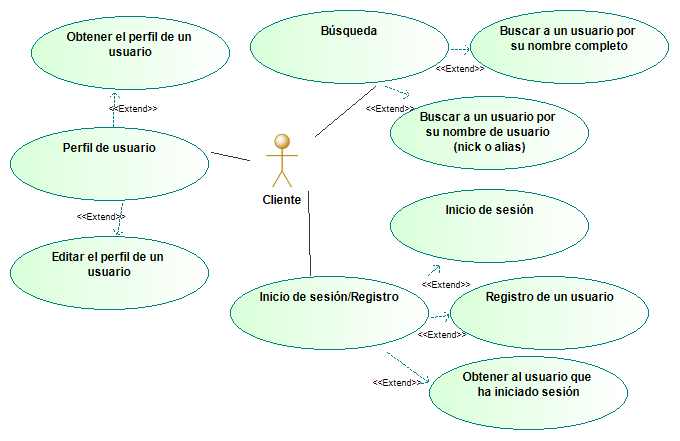
\includegraphics[scale=0.3]{C:/Users/agust/Desktop/UseCaseDiagram_2}

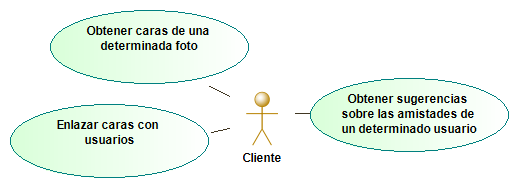
\includegraphics[scale=0.3]{FaceDiagram}

\caption{Diagrama de casos de uso \label{fig:Diagrama-de-casos}}
\end{figure}


\section{Recursos utilizados}

Antes de finalizar el análisis del proyecto desarrollado, es necesario
hablar sobre los recursos utilizados. Ya se detallo anteriormente
las herramientas utilizadas en este proyecto. Pero han sido necesarios
otros recursos importantes para poder llevar a cabo este proyecto.

\subsection{Servidor Virtual Privado (VPS)}

Antes de entrar en detalles, comencemos en una pequeña definición
extraída del soporte de GoDaddy\cite{GoDaddy}, un distinguido proveedor
de alojamientos web y dominios:\cite[Al ocupar el espacio entre los formatos de alojamiento dedicado y compartido, un servidor virtual privado (VPS, por sus siglas en inglés) ofrece muchas de las capacidades y funciones de los servidores dedicados, incluyendo acceso a administrador (raíz) y direcciones IP dedicadas, pero a un precio mucho más bajo][]{ServidoresVPSGoDaddy}.
Es decir, un VPS no es más que un servidor dedicado de menos coste
compartido con otros usuarios. Así que se decidió que podría ser una
buena elección. En mi caso, el servidor no se contrató en GoDaddy,
si no a una empresa francesa llamada OVH, proveedora de alojamiento
web y dominios\cite{OVH}. Lo que quiero destacar de haber contratado
el alojamiento de la aplicación en dicha empresa es que consta con
una interfaz de gestión para el cliente impecable, con una gran usabilidad
y con un diseño acorde al estilo de la pagina web de la empresa. Ademas,
dicha interfaz hace posible poder reinstalar el servidor entero, reiniciarlo,
cambiar de propietario, la posibilidad de mejorar el VPS. Además,
de información relativa al servidor como la localización, su IP, quien
es el administrador, el tipo de SO, el estado del servidor, etc.

A la hora de contratar el servidor se le pide al cliente que Sistema
Operativo utilizar, se selecciona y la empresa te proporciona las
herramientas necesarias para empezar a utilizarlo. De hecho, este
fue uno de los primeros pasos cuando se quiso abordar el problema
especificado anteriormente, el contratar un alojamiento web.

\subsubsection*{Tomcat 8}

Para que fuese posible el despliegue de la API REST desarrollada en
Spring, era necesario un contenedor web donde poder desplegarla. Tomcat
da la capacidad de desplegar aplicaciones web que vienen empaquetadas
en formato WAR o JAR, dependiendo de lo que se quiera hacer. Tomcat
provee un administrador donde poder ver las aplicaciones que se tienen
desplegadas y su ruta de acceso. Por eso, mientras que en el local,
durante el desarrollo en local de la aplicación se accede a la propia
maquina (http://localhost:8080), en producción se accede a la API
a través de la IP remota del VPS, apuntando al puerto correspondiente
y haciendo referencia a la aplicación web desplegada (http://IP:8080/APP).
Tomcat casi siempre va en combinación de Apache, con el objetivo de
configurar el proxy, del cual hablaremos más adelante. La instalación
de Tomcat 8 también fue uno de los primeros pasos a la hora de abordar
el problema.

\subsubsection*{Python, Anaconda y librerías}

Ya se ha hablado de que se tiene como objetivo incluir una mejora
a la aplicación web que tenga relación con la Visión Virtual. Y: ¿qué
es la Visión Artificial sin Python? Cabe destacar que el VPS tenia
Python instalado. Cambien hay que destacar que existen distribuciones
de Python, especializadas en aprendizaje automático entre otros campos.
Además con Anaconda ya no es necesario utilizar el comando pip que
se utiliza con Python para la instalación de librerías, se utiliza
el comando conda.

Por otra parte, para poder proceder con el desarrollo, fue necesario
la instalación de librerías relacionadas con la conexión a la Base
de Datos (mysql), con el framework que permite el desarrollar la API
en Python (bottle), con la lectura de directorios y archivos del servidor
(os), con el reconocimiento facial (face\_recognition), con el deep
learning (dlib), etc. 

\subsection{Dominio y certificado SSL}

Acceder a la aplicación web a través de la IP no es seguro, así que
se decidió la contratación de un dominio acompañado del cifrado SSL
pertinente. Primero se procedió a registrar el nombre del dominio.
Se realizó a través de la misma empresa donde se contrató el servidor.
Después de la contratación, simplemente se creo un registro de tipo
A apuntando a la IP del VPS para poder acceder directamente al dominio.

Por otra parte, por mucho dominio que se tuviese, era necesario que
las peticiones y las respuesta estuviesen cifradas. Así que, a través
de Let's Encrypt \cite{LetsEncrypt}, empresa encargada de proveer
certificados SSL gratuitos, se cifró el trafico de la API y el lado
cliente.

Al igual que con el servidor privado, la interfaz de gestión que proporciona
OVH, da la funcionalidad necesaria para poder administrar el dominio.
La creación, edición y eliminación de registros relacionados con el
dominio, gracias a esto se ha conseguido apuntar el dominio a la IP
consultar los servidores DNS, realizar redirecciones, etc.

\subsection{Otros recursos}

Aparte de lo ya mencionado, han sido necesarios otros recursos para
el correcto funcionamiento de la aplicación. Después de contratar
el dominio y enlazarlo con la IP correspondiente, se presento el problema
de que era necesario utilizar el puerto 8080 para poder acceder a
la API. Por tanto, fue necesario la instalación de Apache con el fin
de configurar un proxy que recibiese todo el tráfico de la API y así
poder eliminar el puerto del dominio.

Para realizar la conexión remota con el servidor y poder realizar
labores administrativas en el mismo e instalar muchos de los recursos
nombrados anteriormente fue necesario SSH. Mediante un programa llamado
PuTTY me fue posible la conexión remota desde cualquier dispositivo.
Ahora bien, en este caso concreto, la empresa a la cual se le contrato
el servidor provee la funcionalidad dentro de su Interfaz de Gestión
de poder conectarse al servidor con un simple click, así que en cierta
manera se podría prescindir de este recurso.

\chapter{Diseño e implementación}

Después del análisis del proyecto, se procede a explicar como se ha
realizado el diseño e implementación de la solución al problema presentado
al principio de este documento. 

\section{Herramientas utilizadas}

En el capitulo de Análisis, concretamente en el capitulo de recursos
utilizados, se entro un poco en detalle de las herramientas utilizadas.
En esta sección se hablará más en detalle de ello.

\subsection{Hardware}

Dado que se trata del desarrollo de una aplicación software, las herramientas
hardware utilizados han sido escasas en número. Entre las herramientas
hardware utilizadas, se encuentran: 
\begin{itemize}
\item Ordenador de sobremesa. Componentes a destacar:
\begin{itemize}
\item \textbf{Procesador} \textbf{(CPU):} AMD Ryzen 3 1300X 3.7Ghz
\item \textbf{Tarjeta gráfica (GPU)}: Asus GeForce GTX 1060 OC Dual 3GB
GDDR5
\item \textbf{Memoria RAM:} Crucial DDR4 2133 PC4-17000 8GB CL15
\item \textbf{Disco Duro:} Seagate BarraCuda 3.5\textquotedbl{} 1TB SATA3
\end{itemize}
\item Ordenador portátil ASUS. Componentes a destacar:
\begin{itemize}
\item \textbf{Procesador} \textbf{(CPU):} Intel Core i5-6300HQ
\item \textbf{Tarjeta gráfica (GPU)}: Nvidia GeForce GTX 950M
\end{itemize}
\item Monitor Samsung 32''.
\end{itemize}

\subsection{Software}

Al contrario que en la subsección anterior, aquí las herramientas
software utilizadas son abundantes. A continuación se procede a detallar
dichas herramientas:

\subsubsection{GitHub y SmartGit}

Antes de hablar de estas herramientas, creo necesario hablar de Git.
Herramienta que ha supuesto un pilar muy importante para el desarrollo
del proyecto. Git es una herramienta de control de versiones. Es especialmente
recomendable cuando el mismo código es utilizado por mas de una persona,
dado que tiene una herramienta para la solución de conflictos. En
mi caso, es cierto que el proyecto a realizar tenia algún tipo de
relación con una de mis compañeras, pero dado que nuestras partes
en el desarrollo están perfectamente parceladas, prácticamente ninguno
de los dos tocaba el trabajo del otro. 

Por otra parte, en mi caso he necesitado Git para poder tener constancia
de versiones estables de la aplicación, y sobre todo para tener un
registro de lo que se ha haciendo y de los avances durante el tiempo
que ha durado el desarrollo.

En otro orden de cosas, GitHub es un sitio web donde alojar proyectos
que han sido desarrollados colaborativamente. En mi caso, usé GitHub
para poder alojar el proyecto y poder hacer uso de él. Consta de una
documentación impecable y proporciona una serie de facilidades que
muchas otras no ofrecen. Después de subir el proyecto y por tanto
crear un repositorio, GitHub te proporciona una URL pública con la
que cualquiera puede acceder y revisar el código.

Por último, tenemos SmartGit. SmartGit es un cliente con interfaz
gráfica para Git, y obviamente tiene la posibilidad de conectar con
GitHub y los repositorios. Con esta herramienta, fui capaz de hacer
todas las operaciones de Git (commit, push, pull, etc.) y de tener
un control gráfico del proyecto. Simplemente proporcionando la URL
del repositorio en GitHub, es posible tener el control del mismo desde
el cliente. Cabe destacar que dicho cliente no es un sitio web, si
no una aplicación de escritorio, por lo que resulta más útil a la
hora de hacer uso de ella.

\subsubsection{Lenguaje de programación y framework.}

El lenguaje de programación que se ha utilizado ha sido Java. Una
de las razones principales fue que se decidió utilizar Spring, como
framework de Java para el desarrollo web. Spring trae consigo una
serie de módulos para hacer más sencillo aún el desarrollo de la aplicación
web. En mi caso, he utilizado los módulos de Spring: Spring Boot,
Spring Data y Spring MVC. Gracias a Spring y a sus módulos, fue posible
no solamente el desarrollo de los controladores encargados de atender
las peticiones HTTP desde el lado del cliente, si no ademas establecer
la configuración de ciertas funcionalidades de la aplicación web. 

A parte de los módulos enumerados anteriormente, se utilizó otro más
Spring Security. Spring Security es el modulo de Spring encargado
de la seguridad de la aplicación. Gracias a dicho módulo se ha sido
capaz de:
\begin{itemize}
\item Establecer la configuración CORS (Intercambio de Recursos de Origen
Cruzado), 
\item Establecer una blacklist de endpoints 
\item Establecer los endpoints que necesitan autenticación para acceder
a ellos
\item Establecer qué mecanismo se seguirá para el inicio de sesión
\item Encriptación de datos sensibles
\end{itemize}
Spring, además, gracias a los modulos mencionados anteriormente, abstrae
al desarrollador de la creación de las tablas a la hora de la persistencia
con la Base de Datos. Me bastó con crear las clases necesarias, anotar
dichas clases para asegurar que Spring hiciese la conversión, y con
desplegar la aplicación, las clases eran transcritas a tablas en la
Base de Datos.

En otro orden de cosas, no solo se ha utilizado Java. Dado que se
quiere hacer uso de la Visión Artificial para incluir una mejora a
la API, se usa Python. La idea es construir otra API con Python, que
proporcione servicios relacionados con el reconocimiento facial. A
raíz del uso de Python para incluir dichas mejoras, fueron necesarias
el uso de varias librerías. A destacar tenemos:
\begin{itemize}
\item Librería relacionada con la conexión a la Base de Datos. Dado que
es necesario que se pudiese acceder a la Base de Datos, tanto para
consulta como para escritura, fue necesario el uso de esta librería.
(mysql.connector \cite{MySQLConnectorPython}
\item Librería relacionada con el reconocimiento facial. (face\_recognition
\cite{FaceRecognitionLibrary})
\item Librería relacionada con la validación de los token JWT. (PyJWT \cite{JWTPythonLibrary}) 
\item OpenCV. Librería relacionada con la Visión Artificial. (cv2 \cite{OpenCV})
\item Framework web para el desarrollo de la API en Python (bottle \cite{Bottle})
\end{itemize}
Se podría decir, que estas herramientas han sido las mas importantes
a la hora del desarrollo de la aplicación. Gracias a ellas, ha sido
posible abordar prácticamente todos los problemas planteados y así
poder llegar a una solución.

\subsubsection{Entorno de programación}

Después de la subsección anterior, se podría intuir qué entorno de
programación es el utilizado en este proyecto. El entorno de programación
utilizado es STS (Spring Tool Suite). STS es un entorno de programación
derivado de Eclipse enfocado especialmente al desarrollo de aplicaciones
en Spring Framework. Se decidió utilizar este entorno de programación
para el desarrollo porque este proyecto no es el primero que se aborda,
durante la carrera he tenido que realizar desarrollos similares y
este entorno es el ideal si se decide utilizar Spring como framework
para el desarrollo. Dicho entorno de programación, al igual que cuando
es necesario utilizar Eclipse, requiere tener instalado Java y Java
JDK. 

Además, se fue capaz de desplegar la aplicación en local para la prueba
de la misma, simulando su puesta en funcionamiento en producción.
Una vez que se desarrollaba una funcionalidad especifica de la API,
se fue capaz de realizar el empaquetamiento de la misma, con el fin
de poner la aplicación en producción. El entorno de programación da
la posibilidad de realizar el empaquetamiento ajustando un par de
opciones. 

Por otra parte, al igual que Eclipse, proporciona soporte para test
unitarios, utilizando Spring para ello. En una de las subsecciones
anteriores se ha hablado de Git para el control de versiones, esta
herramienta me ha permitido realizar operaciones de Git desde el propio
entorno. Además, se indica junto al proyecto en cada momento la rama
en la que te encuentras y el repositorio actual.

Por último, tenemos PyCharm. Entorno de programación especializado
en Python. Dado que se pretende realizar tareas de Visión Artificial
que implican el uso de Python, es necesario el uso de PyCharm. Permite
configurar un entorno de Anaconda para la ejecución del codigo. Además,
da la capacidad de instalar paquetes de Python desde las opciones
del proyecto, tiene una potente herramienta para depurar el código,
etc.

\subsubsection{Gestor de la Base de Datos.}

Dado que se trata de una Base de Datos MariaDB, fue necesario una
herramienta que facilitase la gestión de dicha Base de Datos. Después
de instalar MySQL en el VPS, se decidió el uso de DBeaver. DBeaver
es una herramienta de gestión de Bases de Datos MySQL, de código libre
y con una interfaz de usuario muy intuitiva. Basta con elegir qué
tipo de Base de Datos se quiere gestionar y especificar los datos
de conexión. La herramienta hace lo demás. Con esta herramienta, he
sido capaz de hacer cambios en la Base de Datos permitiendo la posibilidad
de tanto hacerlo mediante la interfaz de gestión como de ejecutar
sentencias SQL que la herramienta se encarga de gestionar.

\section{Arquitectura del software}

En esta sección se describirán cada una de las partes de la solución
que se desarrolla. Indicaré las características en cada subsección,
separando dicha sección por el tipo de API de la que se hable. 

\subsection{Spring API REST}

En esta subsección se va a entrar en detalle sobre la API REST desarrollada
con ayuda de Spring Framework. Como introducción podemos ver en la
Figura \ref{fig:Estructura-del-proyecto} la estructura del proyecto,
organizada por paquetes para mantener la mantenibilidad del código.
Como ya se dijo en capítulos anteriores junto al nombre del proyecto
se indica el repositorio y la rama actual. En un proyecto en Spring
Boot, se distinguen tres carpetas principales ``src/main/java'',
``src/main/resources'' y ``src/test/java''. En la primera carpeta
se encuentra el código fuente de la aplicación, eso es, la funcionalidad
completa de la aplicación. En la segunda carpeta se encuentran los
recursos estáticos (ficheros .js, .css, .png, etc) y las plantillas
de la aplicación si las hubiese, además del fichero de configuración
``application.properties'' del que se hablará más adelante.

\begin{figure}[t]

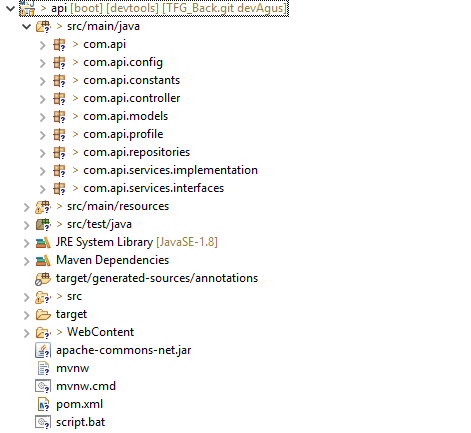
\includegraphics{ProjectStructure.PNG}

\caption{Estructura del proyecto \label{fig:Estructura-del-proyecto}}

\end{figure}

La estructura de toda API REST desarrollada en Spring tiene la estructura
que se ve en la Figura \ref{fig:Diagrama-API-REST}. A lo largo del
capítulo se irá haciendo referencia a dicha figura con el objetivo
de ir explicando cada una de las partes.

\begin{figure}[t]

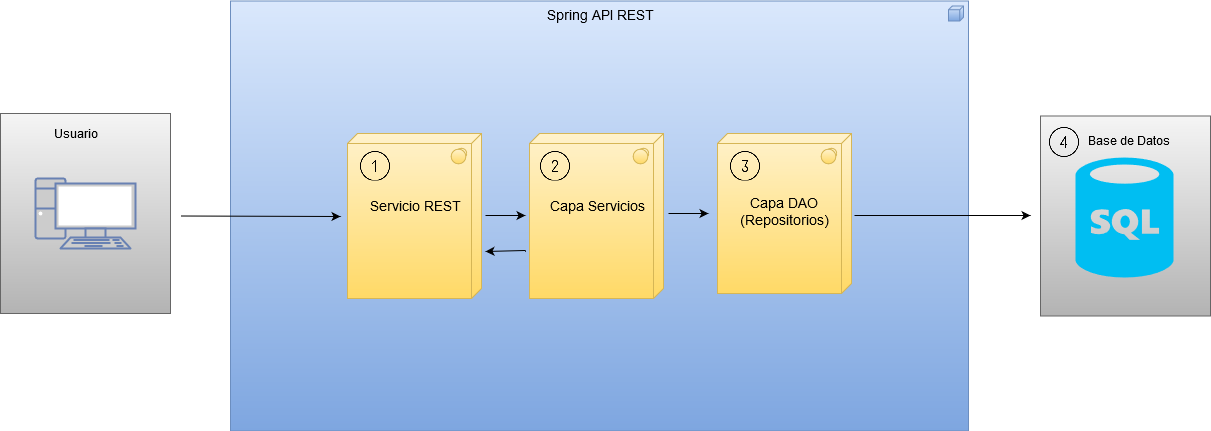
\includegraphics[scale=0.35]{Spring}

\caption{Diagrama API REST en Spring \label{fig:Diagrama-API-REST}}

\end{figure}

\textbf{Spring IoC Container y los beans}

Antes de entrar en detalle sobre cada una de las partes de la aplicación,
es necesario explicar cómo Spring es capaz de realizar todo lo que
se va a ver en futuras secciones. En primer lugar, se tienen los beans.
Los beans son los objetos que componen la columna vertebral de la
aplicación y son administrados por el contenedor de Spring (Spring
IoC Container). Cabe destacar que un bean podría ser un controlador,
acceso a la base de datos, configuración de la seguridad de la aplicación,
etc. Es decir, los beans son los objetos que contienen la funcionalidad
de la aplicación y son configurados por el contenedor de Spring. El
contenedor cuenta con el principio de IoC (Inversion of Control) también
conocido como Inyección de Dependencias. Es un proceso en el cual
los objetos definen sus dependencias, esto es, otros objetos con los
que trabajan dichos objetos, los argumentos del constructor, propiedades
que se establecen en la instancia del o

Ahora bien, gracias a Spring Data, el tipo de Base de Datos que se
utilice es independiente de los repositorios. Bastaría con cambiar
la configuración que se ve en la Figura \ref{fig:Fichero-de-configuraci=0000F3n}.
y se podría utilizar otro tipo de Base de Datos. bjeto despues de
que se construye, etc..

El contenedor de Spring sabe qué objetos instanciar, configurar o
ensamblar gracias a los metadatos de configuración. Estos metadatos
de configuración estan representados a su vez por un fichero XML,
por anotaciones Java o por código Java. El contenedor de Spring esta
representado por la interfaz BeanFactory y ApplicationContext. La
interfaz BeanFactory provee un mecanismo avanzado de configuración
capaz de administrar cualquier objeto, ApplicationContext es una interfaz
que implementa BeanFactory y además de las características propias
de la interfaz BeanFactory, implementa una serie de características
mas avanzadas para el manejo de otro tipo de servicios.

En resumen, el desarrollador provee a través de un fichero XML, mediante
anotaciones o mediante código Java, los beans que necesita el contenedor
de Spring. Dicho contenedor se encargar de tomar esos beans y configurarlos,
ensamblarlos e instanciarlos. Si nos fijamos en la Figura \ref{fig:Diagrama-API-REST},
el contenedor Spring seria el recuadro azul, esto es, la base sobre
la construye todo lo demás.

\subsubsection{Modelos}

Como ya se ha introducido en la sección de las herramientas utilizadas
durante el desarrollo, Spring abstrae al desarrollador de la transcripción
de las clases a las tablas en la Base de Datos. Por lo que tenemos
modelos basados en datos. Suponiendo que se tiene configurada la conexión
con la Base de Datos, en cuanto la aplicación es desplegada es posible
establecer determinadas opciones para la creación de las tablas correspondientes
y los datos contenidos en dichas tablas. 

Para poder realizar la creación de estas tablas, es necesario la creación
de clases con una serie de anotaciones. Se tienen que anotar las clases
con el objetivo de constituyan una entidad y puedan ser traducidas
a tablas de la Base de Datos. Además, hace falta especificar cuál
será la clave primaria de la entidad. Posteriormente, tanto en desarrollo
local como en producción, una vez desplegada la aplicación, Spring
usando lo especificado en un fichero de configuración del que se hablará
más adelante, establece la conexión con la Base de Datos, traduciendo
las relaciones entre clases y las propias clases anotadas pertinentemente
en tablas, con sus claves primarias y foráneas en el caso de que existan
relaciones.

La estructura de los modelos queda representada en la Figura \ref{fig:Diagrama-Entidad-Relaci=0000F3n}.
Entrando más en detalle sobre dichos modelos tenemos:
\begin{itemize}
\item Clase Usuario. Podría decirse que es la entidad central de la aplicación.
Un usuario puede poseer:
\begin{itemize}
\item N publicaciones
\item N comentarios
\item N imágenes provenientes de las sus propias publicaciones
\item N amigos 
\item N caras procedentes de sus imágenes.
\end{itemize}
\item Clase Publicación. Una publicación se compone de imágenes y comentarios.
\item Clase Comentario. Un comentario solamente puede pertenecer a un usuario
y a una publicación.
\item Clase Cara. Las caras procedentes de las fotos, solo puede provenir
de una sola foto y pueden pertenecer a un solo usuario. Cabe destacar
que, estas caras que pertenecen al usuario son caras que se han extraido
de imagenes contenidas en publicación que el propio usuario ha subido.
Está claro que, solamente serán caras de amistades del usuario.
\item Clase Imagen. La clase Imagen solo puede pertenecer a una publicación
y a un usuario. Además puede poseer N caras extraídas de la propia
foto.
\end{itemize}
\begin{figure}[t]
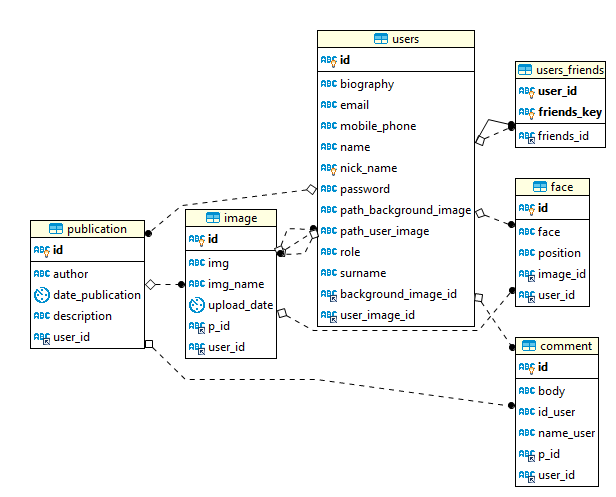
\includegraphics[scale=0.7]{ERDiagramBD}

\caption{Diagrama Entidad-Relación \label{fig:Diagrama-Entidad-Relaci=0000F3n}}

\end{figure}


\subsubsection{Controladores}

Los controladores de la aplicación contienen toda la funcionalidad
de la aplicación. Son el punto de acceso al que el cliente puede acceder
para obtener los recursos que necesita. En este caso, pasa parecido
que con los modelos. Es necesario anotar la clase de cierta manera,
para que Spring sepa que una clase es un controlador que tiene como
objetivo atender la solicitud de recursos que hace el lado cliente.
Si nos fijamos en la Figura \ref{fig:Diagrama-API-REST} se tiene
que los controladores serian el Servicio REST (1). Se trata del punto
de acceso que tiene el lado cliente para poder acceder a los recursos
que necesita.

De este modo, una clase anotada como controlador, contendrá en su
interior una serie de método que se encargara de proveer recursos
al lado cliente. Cada método estará anotado pertinentemente. Por cada
método, es necesario decir qué tipo de método es (GET, POST, DELETE,
PATCH, etc) y qué ruta atiende. Además, si la petición HTTP envia
parámetros en la URL, Spring provee de funcionalidad para poder recoger
estos parámetros y utilizarlos para los fines que se crean necesarios. 

Spring tiene la capacidad de serializar la información que se devuelve
al lado cliente. Siempre y cuando esta información sea serializable.
Por lo que, basta con crear una clase con atributos que sean serializables,
al crear una instancia de ese objeto y devolverlo, Spring haciendo
uso del serializador Jackson devolverá el objeto en formato JSON al
lado cliente. De esta forma, si tuviésemos un método GET que se encargase
de devolver un usuario determinado del sistema y suponiendo que la
clase Usuario contiene atributos serializables, la instancia de la
clase Usuario que se debe devolver, sera serializada y será devuelta
en formato JSON al lado cliente.

Por otra parte, la información que proviene del lado cliente puede
ser interpretada por Spring. Si un método de tipo POST determinado
recibiese un objeto de la clase Usuario, bastaría con añadir un argumento
al método anotado debidamente, de esta forma, Spring se encargará
de formar el objeto de dicha clase con la información en formato JSON
proveniente del lado cliente.

Ahora bien, los controladores que existen en la aplicación son:
\begin{itemize}
\item Controlador de usuarios. Este controlador se encarga de proveer recursos
relacionados con los usuarios. Y, en concordancia con los requisitos
funcionales especificados en el capitulo de Análisis, tenemos:
\begin{itemize}
\item Obtener todos los usuarios.
\item Obtener a un usuario dado su identificador.
\item Editar a un usuario.
\item Eliminar a un usuario.
\item Creación de un usuario.
\end{itemize}
\item Controlador de publicaciones
\begin{itemize}
\item Obtener todas las publicaciones
\item Obtener una publicación dado su identificador
\item Editar una publicación
\item Eliminar una publicación
\item Añadir una publicación
\end{itemize}
\item Controlador de comentarios
\begin{itemize}
\item Obtener todos los comentarios
\item Obtener un comentario dado su identificador
\item Editar un comentario
\item Eliminar un comentario
\item Añadir un comentario
\end{itemize}
\item Controlador encargado de la pagina principal de la aplicación. 
\begin{itemize}
\item Carga de la página principal del lado servidor.
\end{itemize}
\item Controlador encargado del registro y del inicio de sesión
\begin{itemize}
\item Registrar a un usuario
\item Iniciar sesión de un determinado usuario
\item Obtener el usuario que ha iniciado sesión
\end{itemize}
\item Controlador encargado de los amigos
\begin{itemize}
\item Obtener todos los amigos
\item Añadir a un amigo
\item Eliminar a un amigo
\item Obtener las publicaciones de tus amigos.
\item Obtener sugerencias de usuarios que podrian ser amistades
\end{itemize}
\item Controlador de utilidades
\begin{itemize}
\item Búsqueda de un usuario dado su nombre de usuario
\item Búsqueda de usuarios dado su nombre
\end{itemize}
\item Controlador del perfil de usuario
\begin{itemize}
\item Obtener un determinado perfil de usuario
\item Editar perfil de usuario
\end{itemize}
\item Controlador de la descarga de imagenes
\begin{itemize}
\item Obtener una imagen determinada
\end{itemize}
\end{itemize}

\subsubsection{Documentación}

Para la documentación, se usa un módulo de Spring llamado Springfox
Swagger2. Este módulo da la capacidad de realizar la documentación
completa de la API en formato JSON de forma automatizada, basta con
decirle en que paquete están alojadas los controladores de la aplicación.
En cuanto se configura el módulo, indicando dónde se encuentran los
controladores y se despliega la aplicación, se habilita un endpoint
donde poder acceder y poder descargar la documentación en formato
JSON.

Aparte de esto, existe otro modulo derivado del anterior llamado Springfox
Swagger UI, este módulo sigue el mismo proceso de generación de la
documentación que el modulo anterior, la diferencia es que habilita
un endpoint donde es posible ver la documentación gráficamente en
formato HTML y da la capacidad de probar toda la funcionalidad desde
dicha página. Además, como se especificará más adelante, hay endpoints
en los cuales hace falta iniciar sesión previamente, dicho modulo
permite simular dicho inicio de sesión y poder probar todos los endpoints.

Si se accede a la dirección base de la aplicación seguido de ``/swagger-ui.html''
se puede ver la documentación al completo, ordenando los métodos HTTP
por controlador. Una vez se tiene todo configurado, se despliega la
aplicación, y se accede al endpoint habilitado por el propio modulo,
el resultado se puede ver en la Figura \ref{fig:Swagger-UI}, extraida
de la documentación de SpringFox \cite{SpringFox}

\begin{figure}[t]
\includegraphics[scale=0.45]{\string"Swagger UI\string".png}

\caption{Swagger UI \label{fig:Swagger-UI}}

\end{figure}


\subsubsection{Configuración y seguridad de la aplicación web}

Ya se introdujo en la sección de las herramientas utilizadas el uso
de Spring Security para asegurar la seguridad de la aplicación y además
es necesaria la configuración de la documentación, como ya se entró
en detalle anteriormente.

Ahora bien, para poder hacer que todo esto funcione, es necesario
la configuración a través de clases anotadas pertinentemente. En total,
se tienen 3 clases que se encargan de la configuración de la seguridad
de la aplicación:
\begin{itemize}
\item Clase relacionada con la configuración de la seguridad de la web.
En esta clase, se establecen configuraciones básicas sobre la seguridad
de la aplicación. Se establece la encriptación de la contraseña de
los usuarios, se establece la configuración CORS de la aplicación
con el fin de una comunicación existosa del lado cliente.
\item Clase relacionada con el acceso a los recursos de la aplicación. En
esta clase, se establece una lista blanca y una lista negra de puntos
de acceso para el lado cliente. Básicamente, se establecen los recursos
a los que el lado del cliente puede acceder y a los que necesita antes
autenticación para poder acceder.
\item Clase relacionada con la autenticación basada en un token JWT. En
esta clase, se establece la configuración de la autorización con token. 
\begin{itemize}
\item El tipo de autenticación que se usa en al aplicación es OAuth2.0 y
JWT (JSON Web Tokens). Estos servicios proveen al lado cliente el
acceso a los recursos de forma limitada, siempre y cuando se proporcionen
los datos de autenticación pertinentes. Sabiendo el flujo del token
JWT usando OAuth2.0 \cite{FlujoTokenJWT}, el lado cliente puede acceder
a los recursos con la debida autenticación. Concretamente se usa OAuth2.0
Password Grant Type. Como se ve en el flujo de datos mostrado en la
Figura \ref{fig:Flujo-de-datos} \ref{fig:Flujo-de-datos}proporcionado
por la documentación de Oracle \cite{OAuth}, se habilita un endpoint,
dado por la propia dependencia de OAuth, al cual es necesario hacer
una petición POST con una serie de parámetros que necesita OAuth para
realizar la autenticacion. Estos parámetros los establece OAuth, pero
los valores los pone el lado del servidor y los comparte con el lado
del cliente. 
\item El usuario introduce su usuario y contraseña (previo registro), el
lado del cliente realiza una petición a dicho endpoint con los parametros
pertinentes para obtener el token y a partir de ahí, el cliente debe
de mandar el token en cada petición que se haga para confirmar que
el usuario sigue autentificado. El token tiene un tiempo de expiración
de 12 horas establecido por la propia API. Ahora bien, dentro de la
aplicación existe un fichero de configuración, del cual se entrara
en detalle más adelante. En dicho fichero se establecen los valores
para los parametros que necesita OAuth. En esta clase, se toman esos
valores dados en el fichero y se establece la autenticación OAuth
con la que el cliente debe acceder.
\end{itemize}
\end{itemize}
\begin{figure}[t]

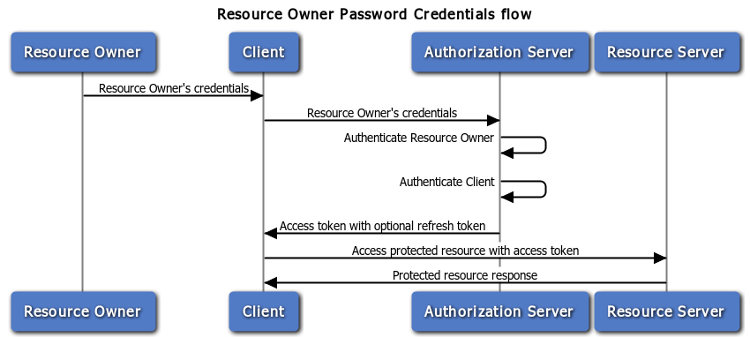
\includegraphics[scale=0.6]{OAuthTokenJWTSequenceDiagram}

\caption{Flujo de datos de OAuth2.0 con token JWT\label{fig:Flujo-de-datos}}

\end{figure}

Además, Spring permite configurar la aplicación web desde un fichero
dentro del propio proyecto. En mi caso el fichero se denomina ``application.properties'',
en dicho fichero van parametros de configuración globales. En dicho
fichero, se especifican los parámetros que necesita Spring para la
autenticación mediante OAuth2.0.

\subsubsection{Repositorios}

Los repositorios o DAOs (Data Access Object) son las herramientas
que se encargan de la persistencia de la aplicación. Proporcionan
una capa de abstracción para el desarrollador, abstrayendolo de las
consultas SQL requeridas para poder añadir, consultar o eliminar datos
de la Base de Datos.

La interfaz JpaRepository contiene una serie de métodos básicos que
implementan todas las operaciones que se pueden realizar (crear, leer,
actualizar y eliminar) con respecto a la Base de Datos. Además es
posible que el desarrollador pretenda realizar consultas cambiando
el criterio de búsqueda, para ello, simplemente se crea la cabecera
del método en la interfaz. El nombre del método debe de seguir un
formato concreto: Debe empezar por ``findBy'' seguido del atributo
de la clase por el que se quiere buscar. Debe pasarse por parámetro
el atributo por el que se quiere buscar, con el tipo adecuado. Si
el objeto que se devuelve no es una lista, quiere decir que el método
encontrará uno y lo devolverá. En cambio si se devuelve una lista,
el método buscara todas las ocurrencias del valor del parámetro que
se le pase.

Un solo repositorio no va a poder hacerse cargo de todos los modelos
de la aplicación, ya que cada repositorio se asocia al tipo del modelo
sobre el que se quieren realizar una serie de operaciones.

Haciendo referencia a la Figura \ref{fig:Diagrama-API-REST}, se trata
de los Repositorios (3) o DAOs. Es la ultima puerta que se cruza para
almacenar la información en la Base de Datos. 

\subsubsection{Servicios}

A diferencia del apartado anterior, los servicios no es una herramienta
proporcionada por Spring. Se implementa por parte del desarrollador.
En mi caso, he implementado un servicio por cada uno de los repositorios
que existen. Dichos servicios deben ir anotados pertinentemente y
tendrán métodos que implementaran los mismos métodos que el DAO.

El objetivo de la creación de Servicios es proporcionar mantenibilidad
al código. La creación de servicios implican proporcionar una capa
de abstracción para el desarrollador, de manera que si es necesario
cambiar la implementación de algunas de las operaciones de los repositorio,
bastaria con hacer las modificaciones pertinentes en los servicios
sin que el código de los controladores quedase afectado.

Los servicios existentes en la aplicación son los siguientes:
\begin{itemize}
\item Servicio dedicado a los usuarios
\item Servicio dedicado a las publicaciones
\item Servicio dedicado a los comentarios
\item Servicio dedicado a las imagenes
\item Servicio dedicado al servidor donde se aloja la aplicación
\item Servicio dedicado a las caras extraídas de las imagenes
\end{itemize}
Dado que los servicios es una capa que se encuentra entre los controladores
y los repositorios, en la Figura \ref{fig:Diagrama-API-REST}, se
trata de la Capa Servicios (2) y se encarga de mediar entre el Servicio
Rest (1) y los DAOs (3) proporcionando la capa de abstracción de la
que ya se ha hablado.

\subsubsection{Base de Datos}

En el capítulo de Análisis se introdujo un poco a la Base de Datos
dado es unos de los recursos externos utilizados. Se utiliza un sistema
de gestión de Bases de Datos derivado de SQL: MariaDB. Una vez se
configura debidamente en el VPS, en Spring se establece la configuración
global en el fichero ``application.properties'' para que la aplicación
pueda conectarse a la Base de Datos. Además, es necesario realizar
una integración del tipo de Base de Datos en Spring. Para ello existe
una dependencia que se encarga de integrar MariaDB en Spring.

Cabe destacar que se tienen dos bases de datos, una usada para el
desarrollo en local, para pruebas. Y otra para producción, usada en
el despliegue de la aplicación. Una vez más, para cambiar una Base
de Datos por otra basta con indicarlo en el fichero de configuración
nombrado anteriormente

Y por último, haciendo referencia a la Figura \ref{fig:Diagrama-API-REST},
la Base de Datos (4) es el último destino para mantener la persistencia
de la información. Siendo los DAOs (3) los encargados de administrar
el almacenamiento de dicha información.

\subsection{Python API REST}

Como ya se introdujo en anteriores secciones, además de la API REST
desarrollada con Spring Framework, se tiene una API REST desarrollada
a traves de Python y sus librerias dedicadas a la Vision Artificial.
Dicha API provee un servicio especial a la API desarrollada en Spring:
El reconocimiento facial. Además, fue necesaria configurar debidamente
la aplicación, dado que tambien será utilizada por el lado cliente. 

Antes de proceder a la descripción de cada una de las partes del algoritmo,
es necesario aclarar una serie de cuestiones. La libreria usada para
el reconocimiento facial (face\_recognition) se basa en el deep learning,
concretamente mediante el uso de redes neuronales, para el reconocimiento
facial. Dicha libreria no necesita que el desarrollador le provea
un conjunto de test para el correcto reconocimiento de caras en una
foto.

En un primer momento, lo que se pretendia era que un controlador de
la API REST de Spring ejecutase un script de Python que realizase
la funcionalidad. El problema es que esto no fue posible en un entorno
web, por lo que fue necesario la realizacion de una segunda API REST
hecha en Python. Por otra parte, si se presta atención al repositorio
de dicha libreria en GitHub \cite{FaceRecognitionLibrary} se puede
ver que puede usarse junto con un framework web, en este caso se usa
Flask, el cual es muy parecido al usado en este caso.

\subsubsection{Algoritmo}

Como ya se ha dicho, la libreria no necesita ser entrenada para realizar
su cometido. Por lo que basta con proporcionarle una foto y esta nos
devolverá las posiciones de la cara (en pixeles) en la foto. En la
Figura \ref{fig:Diagrama-de-actividad} podemos ver el algoritmo que
se sigue a la hora de subir una foto, representado mediante un diagrama
de actividad se ha incluido el FrontEnd para poder explicar mejor
la utilidad de la API en una aplicación web. El algoritmo que se sigue
es el siguiente, teniendo en cuenta la Figura \ref{fig:Diagrama-de-actividad}:
\begin{enumerate}
\item El usuario se dispone a subir una foto
\item Se muestra una vista previa de la foto
\item Se piden las caras al lado servidor.y si es posible, se piden tambien
sugerencias
\item El lado servidor devuelve caras y puede (o no) devolver sugerencias
\item El lado cliente dibuja las caras en la vista previa, y sugerirá al
usuario si es posible
\item El usuario etiqueta las caras con los usuarios y se lo comunica al
lado servidor a traves del lado cliente
\item El usuario, si está conforme, confirmara la subida de la foto
\item Vuelta al paso 1.
\end{enumerate}
Ahora bien, cabe decir, que el lado servidor devolverá caras siempre
y cuando existan caras en la foto. Si no existen caras en la foto,
no se devolverán, además de no devolver sugerencias como es obvio.
Si es posible devolver caras, el servidor devolverá caras además de
sugerencias dependiendo de las fotos subidas anteriormente por el
usuario. El algoritmo aprende de las caras que el usuario ha registrado
anteriormente. Por lo que, si el usuario sube su primera foto a la
aplicación, es posible que el servidor devuelva caras, pero no devolverá
en ningú caso sugerencias, dado que no tiene registro de fotos y por
tanto no tendrá caras registradas. El usuario solo podra etiquetar
caras con otros usuarios si y solo si estos usuarios pertenecen a
su lista de amigos. En otro caso, no será posible etiquetar.

\begin{figure}[t]

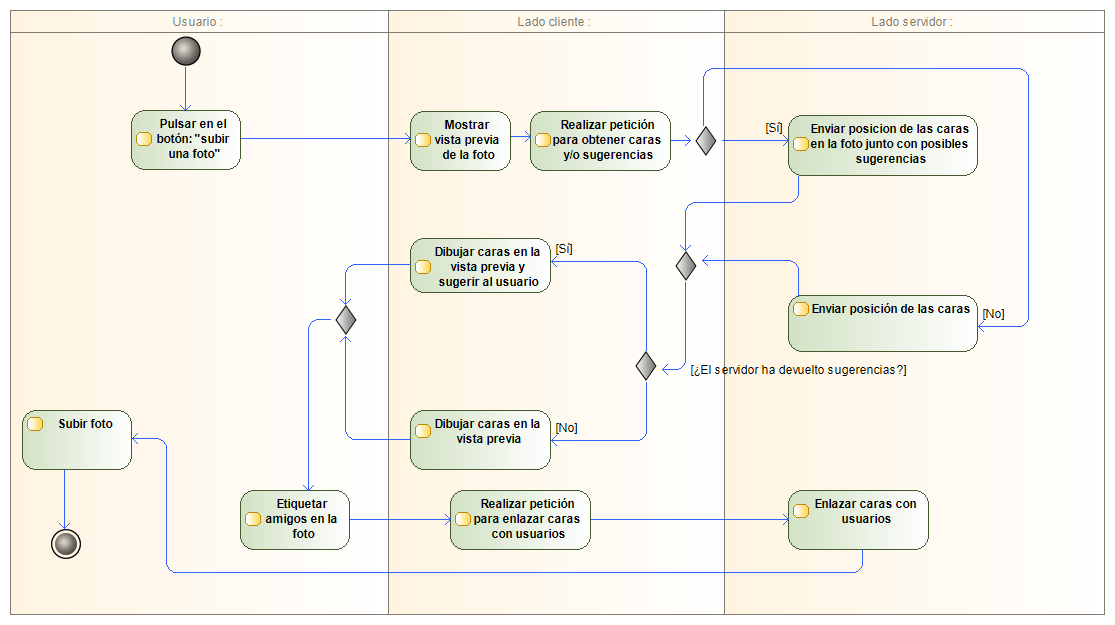
\includegraphics[scale=0.3]{FaceAlgorithm}

\caption{Diagrama de actividad de la subida de fotos\label{fig:Diagrama-de-actividad}}

\end{figure}


\subsubsection{Controladores}

Una vez se ha hablado sobre cómo funciona el algoritmo de reconocimiento,
se procede a hablar de la funcionalidad que hace posible que todo
funcione correctamente. Se tienen dos controladores principales:
\begin{itemize}
\item El controlador encargado de proporcionar caras y sugerencias si es
posible. Haciendo referencia a la Figura \ref{fig:Diagrama-de-actividad},
este método se corresponde con las actividaddes (4) y (6). Al principio,
se encarga de extraer las posiciones de las caras, pero antes de devolver
las posiciones correspondientes, comprueba si hay sugerencias. Por
lo que, por cada cara que se encuentra en la foto, se busca en el
directorio de caras de las amistades del usuario con el objetivo de
encontrar alguna coincidencia y así poder hacer sugerencias. Por lo
que a la vuelta, se devuelve en formato JSON, las posiciones de las
caras (si se encuentran la foto enviada) y las sugerencias de dicha
cara (si se se han encontrado sugerencias de la cara).
\item El controlador encargado de enlazar caras con usuarios. Una vez que
las posiciones de las caras llegan al lado cliente y son pintadas
para que el usuario se encargue de etiquetar las caras con los nombres
de usuario de sus amistades (actividades (5), (6) y (7) en la Figura
\ref{fig:Diagrama-de-actividad}), es necesario que el sistema sepa
qué cara se corresponde con qué usuario. Por lo que una vez se ha
etiquetado (actividad (9) en la Figura \ref{fig:Diagrama-de-actividad}),
se realiza la petición para enlazar las caras con usuario, enviando
al lado servidor desde el lado cliente, la posición de la cara en
la foto, la foto en cuestión y el usuario que se encuentra en esa
cara (actividades (10) y (11) en la Figura \ref{fig:Diagrama-de-actividad}).
\end{itemize}

\subsubsection{CORS}

Al igual que ocurria en la API REST de Spring es necesario realizar
la configuración pertinente del mecanismo CORS (Intercambio de Recursos
de Origen Cruzado) para ello se desarrolla lo que se denomina un decorador
de Python. Un decorador de Python es basicamente una función que es
usada para extender el comportamiento de otra funcion, sin modificar
en nada a dicha función. Por lo que, se realiza un decorador para
los endpoints que se tienen en la API REST que realice la configuración
adecuada, para así poder realizar una comunicación exitosa con el
lado cliente

\subsubsection{Verificación de JWT}

En la sección anterior, se habló de OAuth2.0 y de los JWT que se usan
para la autenticación del usuario en el sistema. Dado que esta API
REST no pertenece a Spring, es necesario comprobar que el usuario
que accede a los recursos esta autenticado. Por lo que, haciendo uso
de la libreria PyJWT se realiza una validación del token que llega
desde el lado cliente. Y se comprueba que el usuario exista en el
sistema. Si todo va bien, se le permite al lado cliente acceder a
los recursos del lado servidor.

\subsubsection{Servidor multi-hilo}

Como se ha visto, el framework Bottle provee toda la funcionalidad
necesaria para la construccion de una API REST en Python. Pero como
se puede comprobar en la documentación de dicha herramienta, no provee
la funcionalidad necesaria para hacer que la aplicación atienda a
mas de una petición concurrentemente. Por lo que, fue necesaria otra
libreria que le provea a Bottle esa funcionalidad de la que carece.
En la documentación de Bottle se recomiendas varias librerias capaces
de realizar dichan funcionalidad como se ve en la Figura \ref{fig:Tabla-de-adaptadores},
se eligió CherryPy como librería para realizar esta función. Como
se pueden ver en la Figura \ref{fig:Tabla-de-adaptadores}, dicha
libreria es bastante estable y realiza la función que necesitamos.
Además, en un primer momento se optó por el uso de paste, da dado
que ademas de la estabilidad, ah sido testado y probado, pero carece
de documentación consistente, por lo que se optó por CherryPy. 

\begin{figure}[t]
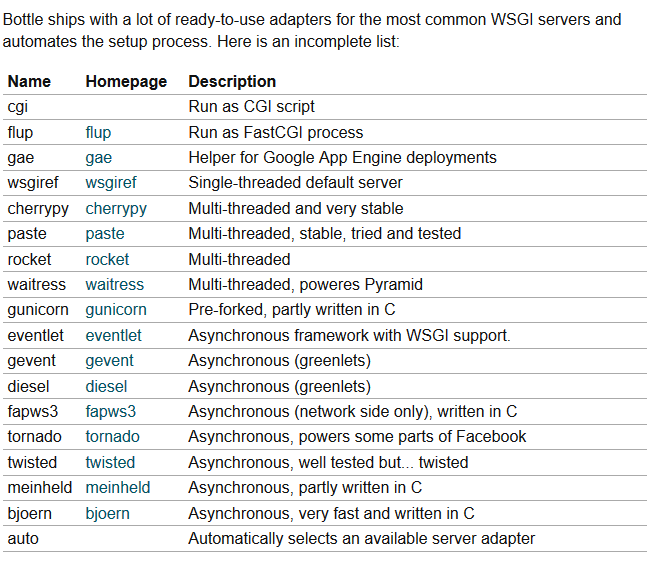
\includegraphics{TablaAdaptadoresBottle.PNG}

\caption{Tabla de adaptadores para Bottle \label{fig:Tabla-de-adaptadores}}
\end{figure}


\chapter{Capítulo de métricas.}

\chapter{Presentación}

\chapter{Conclusiones}

En este capítulo se resumen los objetivos conseguidos, se presentan
las conclusiones y las posibles continuaciones de este trabajo.

\section{Objetivos cumplidos}

\section{Futuros trabajos}

\appendix

\chapter{Guía de instalación de LyxTFT}

Este anexo describe el proceso de instalación de Lyx en diferentes
sistemas operativos.

\section*{\cleardoublepage}

\printbibliography

\printindex
\end{document}
